\documentclass[hidelinks, 11pt, fleqn]{article}   	% use "amsart" instead of "article" for AMSLaTeX format
\usepackage{geometry}                		% See geometry.pdf to learn the layout options. There are lots.
\usepackage{wrapfig}
\usepackage{tikz}
\usetikzlibrary{decorations.pathreplacing}
\usetikzlibrary{calc}
\usepackage{listings}
\usepackage{color}

\definecolor{codegreen}{rgb}{0,0.6,0}
\definecolor{codegray}{rgb}{0.5,0.5,0.5}
\definecolor{lightgray}{rgb}{0.7,0.7,0.7}
\definecolor{codepurple}{rgb}{0.58,0,0.82}
\definecolor{backcolour}{rgb}{0.92,0.92,0.92}

\renewcommand{\lstlistingname}{Algorithm}% Listing -> Algorithm

\lstdefinestyle{mystyle}{
	backgroundcolor=\color{backcolour},   
	commentstyle=\color{codegray},
	keywordstyle=\color{red},
	numberstyle=\tiny\color{lightgray},
	stringstyle=\color{codepurple},
	basicstyle=\footnotesize,
	breakatwhitespace=false,         
	breaklines=true,                 
	captionpos=b,                    
	keepspaces=true,                 
	numbers=left,                    
	numbersep=5pt,                  
	showspaces=false,                
	showstringspaces=false,
	showtabs=false,                  
	tabsize=4
}

\lstset{style=mystyle}

\usepackage{amsmath}
\usepackage{mathtools}
\usepackage{algorithm}
\usepackage{algpseudocode}
\geometry{letterpaper}                   		% ... or a4paper or a5paper or ... 
%\geometry{landscape}                		% Activate for rotated page geometry
%\usepackage[parfill]{parskip}    		% Activate to begin paragraphs with an empty line rather than an indent
\usepackage{graphicx}				% Use pdf, png, jpg, or eps§ with pdflatex; use eps in DVI mode
\usepackage{subcaption}
\usepackage{hyperref}
								% TeX will automatically convert eps --> pdf in pdflatex		
\usepackage{amssymb}

%SetFonts

%SetFonts
\newtagform{brackets}{[}{]}
\usetagform{brackets}

\title{\textbf{Microglider Assembly}}
\author{Patrick Sorn}
%\date{}							% Activate to display a given date or no date

\begin{document}
\newcommand{\hole}[3] % x in cm, y in cm, radius in mm
{ 
	% draw hole
	\draw (#1,#2) circle (#3mm);
	% crosshair
	\draw (#1,#2-0.05) -- (#1,#2+0.05);
	\draw (#1-0.05,#2) -- (#1+0.05,#2);
	% centering lines
	\draw (#1,#2-0.1*#3-0.05) -- (#1,#2-0.1);
	\draw (#1,#2+0.1) -- (#1,#2+0.1*#3+0.05);
	\draw (#1-0.1*#3-0.05,#2) -- (#1-0.1,#2);
	\draw (#1+0.1,#2) -- (#1+0.1*#3+0.05,#2);
}
\newcommand{\dimsv}[3] % start, end, x
{
	\draw (#3-0.2,#1) -- (#3+0.2,#1);
	\draw[<-] (#3,#1) -- (#3,{(#1+#2)/2-0.2});
	\draw (#3,{(#1+#2)/2}) node {\footnotesize \pgfmathparse{(#2 - #1)*10} \pgfmathprintnumber{\pgfmathresult} };
	\draw[->] (#3,{(#1+#2)/2+0.2}) -- (#3,#2);
	\draw (#3-0.2,#2) -- (#3+0.2,#2);
}
\newcommand{\dimsh}[3] % start, end, y
{
	\draw (#1,#3-0.1) -- (#1,#3+0.1);
	\draw[<-] (#1,#3) -- ({(#1+#2)/2-0.3},#3);
	\draw ({(#1+#2)/2},#3) node {\footnotesize \pgfmathparse{(#2 - #1)*10} \pgfmathprintnumber{\pgfmathresult} };
	\draw[->] ({(#1+#2)/2+0.3},#3) -- (#2,#3);
	\draw (#2,#3-0.1) -- (#2,#3+0.1);
}
\maketitle
\tableofcontents 
\pagebreak
\section{Parts}
\subsection{Motor Mount}
Motor Mount (Aluminium):
\begin{figure}[h]
	\begin{tikzpicture}
	% draw bottom front
	\draw[thick] (0,0) -- (0,2) -- (3,2) -- (3,0) -- (0,0);
	\draw[dashed] (0,0.2) -- (3,0.2);
	\hole{0.5}{0.6}{1.5};
	\hole{0.5}{1.6}{1.5};
	\hole{2.5}{0.6}{1.5};
	\hole{2.5}{1.6}{1.5};
	\draw[densely dotted] (0.7,0.6) -- (2.3,0.6);
	\draw[densely dotted] (2.7,0.6) -- (3.1,0.6);
	\draw[densely dotted] (0.7,1.6) -- (2.3,1.6);
	\draw[densely dotted] (2.7,1.6) -- (3.1,1.6);
	\draw[densely dotted] (0.5,0.8) -- (0.5,1.4);
	\draw[densely dotted] (0.5,1.8) -- (0.5,2.3);
	\draw[densely dotted] (2.5,0.8) -- (2.5,1.4);
	\draw[densely dotted] (2.5,1.8) -- (2.5,2.3);
	\dimsv{0.0}{0.6}{3.3};
	\dimsv{0.6}{1.6}{3.3};
	\dimsv{1.6}{2.0}{3.3};
	\dimsv{0.0}{2.0}{3.8};
	\dimsh{0.0}{0.5}{2.3};
	\dimsh{0.5}{2.5}{2.3};
	\dimsh{2.5}{3.0}{2.3};
	\dimsh{0.0}{3.0}{2.6};
	% draw bottom back
	\draw[thick] (5,0) -- (5,2) -- (8,2) -- (8,0) -- (5,0);
	\draw[thick] (5,0.2) -- (8,0.2);
	\hole{5.5}{0.6}{1.5};
	\hole{5.5}{1.6}{1.5};
	\hole{7.5}{0.6}{1.5};
	\hole{7.5}{1.6}{1.5};
	% draw front
	\draw[thick] (0,5) -- (3,5) -- (3,8) -- (0,8) -- (0,5);
	\draw[dashed] (0,5.2) -- (3,5.2);
	\hole{0.7}{5.7}{1.5};
	\hole{0.7}{7.3}{1.5};
	\hole{2.3}{5.7}{1.5};
	\hole{2.3}{7.3}{1.5};
	\hole{1.5}{6.5}{8};
	\draw[densely dotted] (0.9,5.7) -- (2.1,5.7);
	\draw[densely dotted] (2.5,5.7) -- (3.1,5.7);
	\draw[densely dotted] (0.9,7.3) -- (2.1,7.3);
	\draw[densely dotted] (2.5,7.3) -- (3.1,7.3);
	\draw[densely dotted] (2.3,6.5) -- (3.1,6.5);
	\draw[densely dotted] (0.7,4.8) -- (0.7,5.5);
	\draw[densely dotted] (0.7,5.9) -- (0.7,7.1);
	\draw[densely dotted] (1.5,4.8) -- (1.5,5.7);
	\draw[densely dotted] (2.3,4.8) -- (2.3,5.5);
	\draw[densely dotted] (2.3,5.9) -- (2.3,7.1);
	\dimsv{5.0}{5.7}{3.3};
	\dimsv{5.7}{6.5}{3.3};
	\dimsv{6.5}{7.3}{3.3};
	\dimsv{7.3}{8.0}{3.3};
	\dimsv{5.0}{8.0}{3.8};
	\dimsh{0.0}{0.7}{4.7};
	\dimsh{0.7}{1.5}{4.7};
	\dimsh{1.5}{2.3}{4.7};
	\dimsh{2.3}{3.0}{4.7};
	\dimsh{0.0}{3.0}{4.4};
	% draw back
	\draw[thick] (5,5) -- (8,5) -- (8,8) -- (5,8) -- (5,5);
	\draw[thick] (5,5.2) -- (8,5.2);
	\hole{5.7}{5.7}{1.5};
	\hole{5.7}{7.3}{1.5};
	\hole{7.3}{5.7}{1.5};
	\hole{7.3}{7.3}{1.5};
	\hole{6.5}{6.5}{8};
	% draw side left
	\draw[thick] (10,5) -- (12,5) -- (12,5.2) -- (10.2,5.2) -- (10.2,8) -- (10,8) -- (10,5);
	\dimsv{5.0}{8.0}{9.7};
	\dimsh{10.0}{12.0}{4.7};
	% draw side right
	\draw[thick] (14,5) -- (16,5) -- (16,8) -- (15.8,8) -- (15.8,5.2) -- (14,5.2) -- (14,5);
	\end{tikzpicture}
\caption{Motor mount front, rear, bottom and side view.}
\label{fig:motor_mount}
\end{figure}
\newpage
\subsection{Fuselage}
The fuselage is 36cm long, 2mm thick and 4cm wide, consists of aluminium and provides connectivity to sensors and drivers.
The construction plans for the fuselage can be found in figures \ref{fig:fuselage1} and \ref{fig:fuselage2}.
\begin{figure}
	\centering
	\begin{tikzpicture}
	% draw first part border
	\draw[thick] (0,0) -- (0,18.3) -- (4,18.3) -- (4,0);
	\draw[dotted] (0,-1) -- (0,0);
	\draw[dotted] (4,-1) -- (4,0);
	% draw PCA9685
	\hole{1.05}{0.3}{1.375};
	\hole{1.05}{5.9}{1.375};
	\hole{2.95}{0.3}{1.375};
	\hole{2.95}{5.9}{1.375};
	\draw[densely dotted] (1.25,0.3) -- (2.75,0.3);
	\draw[densely dotted] (3.15,0.3) -- (4.1,0.3);
	\draw[densely dotted] (1.25,5.9) -- (2.75,5.9);
	\draw[densely dotted] (3.15,5.9) -- (4.1,5.9);
	\draw[densely dotted] (1.05,-0.1) -- (1.05,0.1);
	\draw[densely dotted] (1.05,0.5) -- (1.05,5.7);
	\draw[densely dotted] (2.95,-0.1) -- (2.95,0.1);
	\draw[densely dotted] (2.95,0.5) -- (2.95,5.7);
	\draw[rounded corners] (1.3,0.15) rectangle (2.7,0.4);
	\draw[rounded corners] (0.5,0.6) rectangle (1.5,5.6);
	\draw[rounded corners] (1.3,5.75) rectangle (2.7,6);
	\draw[rounded corners] (2.5,0.6) rectangle (3.5,5.6);
	%-- (11.5,0.6) -- (11.5,5.6) -- (10.5,5.6) -- (10.5,0.6);
	% draw wing mount
	\hole{1.0}{7.4}{1.5};
	\hole{1.0}{13.4}{1.5};
	\hole{3.0}{7.4}{1.5};
	\hole{3.0}{13.4}{1.5};
	\draw[densely dotted] (1.2,7.4) -- (2.8,7.4);
	\draw[densely dotted] (3.2,7.4) -- (4.1,7.4);
	\draw[densely dotted] (1.2,13.4) -- (2.8,13.4);
	\draw[densely dotted] (3.2,13.4) -- (4.1,13.4);
	\draw[densely dotted] (1.0,7.6) -- (1.0,13.2);
	\draw[densely dotted] (3.0,7.6) -- (3.0,13.2);
	% draw stabilizer mount
	\hole{2.0}{15.9}{1.5};
	\hole{2.0}{17.9}{1.5};
	\draw[densely dotted] (2.2,15.9) -- (4.1,15.9);
	\draw[densely dotted] (2.2,17.9) -- (4.1,17.9);
	\draw[densely dotted] (2.0,16.1) -- (2.0,17.7);
	% description
	% vertical dimensions
	\dimsv{0.0}{0.3}{4.3};
	\dimsv{0.3}{5.9}{4.3};
	\dimsv{5.9}{7.4}{4.3};
	\dimsv{7.4}{13.4}{4.3};
	\dimsv{13.4}{15.9}{4.3};
	\dimsv{15.9}{17.9}{4.3};
	\dimsv{0.0}{18.3}{4.8};
	% horizontal dimensions
	% total
	\dimsh{0.0}{4.0}{-0.4};
	% PCA9685
	\dimsh{0.0}{1.05}{-0.1};
	\dimsh{1.05}{2.95}{-0.1};
	\dimsh{2.95}{4.0}{-0.1};
	% Wing mount
	\dimsh{0.0}{1.0}{7.1};
	\dimsh{1.0}{3.0}{7.1};
	\dimsh{3.0}{4.0}{7.1};
	% Stabilizer mount
	\dimsh{0.0}{2.0}{15.6};
	\dimsh{2.0}{4.0}{15.6};
	% draw sections
	\draw [decorate,decoration={brace,amplitude=10pt},xshift=-4pt,yshift=0pt] (5.5,6.5) -- (5.5,0) node [black, midway, xshift=1.3cm] {\footnotesize PCA9685};
	\draw [decorate,decoration={brace,amplitude=10pt},xshift=-4pt,yshift=0pt] (5.5,14.5) -- (5.5,6.5) node [black, midway, xshift=1.2cm, align=center] {\footnotesize Wing\\\footnotesize Mount};
	\draw [decorate,decoration={brace,amplitude=10pt},xshift=-4pt,yshift=0pt] (5.5,18.3) -- (5.5,14.5) node [black, midway, xshift=1.4cm, align=center] {\footnotesize Stabilizer\\\footnotesize Mount};
	\end{tikzpicture}
	\caption{Fuselage Part 1.}
	\label{fig:fuselage1}
\end{figure}
\begin{figure}
	\centering
	\begin{tikzpicture}
	% draw second part border
	\draw[thick] (0,17.7) -- (0,0) -- (4,0) -- (4,17.7);
	\draw[dotted] (4,17.7) -- (4,19);
	\draw[dotted] (0,17.7) -- (0,19);
	% -- (0,17.7) -- (0,0);
	% draw motor mount holes
	\hole{1.0}{0.6}{1.5};
	\hole{1.0}{1.6}{1.5};
	\hole{3.0}{0.6}{1.5};
	\hole{3.0}{1.6}{1.5};
	\draw[densely dotted] (1.2,0.6) -- (2.8,0.6);
	\draw[densely dotted] (3.2,0.6) -- (4.1,0.6);
	\draw[densely dotted] (1.2,1.6) -- (2.8,1.6);
	\draw[densely dotted] (3.2,1.6) -- (4.1,1.6);
	\draw[densely dotted] (1.0,0.8) -- (1.0,1.4);
	\draw[densely dotted] (3.0,0.8) -- (3.0,1.4);
	% draw raspberry pi zero holes
	\hole{0.85}{2.5}{1.375};
	\hole{0.85}{8.3}{1.375};
	\hole{3.15}{2.5}{1.375};
	\hole{3.15}{8.3}{1.375};
	\draw[densely dotted] (1.05,2.5) -- (2.95,2.5);
	\draw[densely dotted] (3.35,2.5) -- (4.1,2.5);
	\draw[densely dotted] (1.05,8.3) -- (2.95,8.3);
	\draw[densely dotted] (3.35,8.3) -- (4.1,8.3);
	\draw[densely dotted] (0.85,2.7) -- (0.85,8.1);
	\draw[densely dotted] (3.15,2.7) -- (3.15,8.1);
	\draw[rounded corners] (0.5,2.85) rectangle (1.2,8.0);
	\draw[rounded corners] (2.8,2.8) rectangle (3.5,8.0);
	% draw power distribution board
	% draw INA219 holes
	\hole{1.0}{14.0}{1.375};
	\hole{1.0}{15.7}{1.375};
	\hole{3.0}{14.0}{1.375};
	\hole{3.0}{15.7}{1.375};
	\hole{2.0}{14.0}{7};
	\hole{2.0}{15.6}{4};
	\draw[densely dotted] (1.2,14.0) -- (2.8,14.0);
	\draw[densely dotted] (3.2,14.0) -- (4.1,14.0);
	\draw[densely dotted] (1.2,15.7) -- (2.8,15.7);
	\draw[densely dotted] (3.2,15.7) -- (4.1,15.7);
	\draw[densely dotted] (1.0,13) -- (1.0,13.8);
	\draw[densely dotted] (3.0,13) -- (3.0,13.8);
	\draw[densely dotted] (1.0,14.2) -- (1.0,15.5);
	\draw[densely dotted] (3.0,14.2) -- (3.0,15.5);
	% draw MPU9250 holes
	\hole{1.45}{16.7}{1.375};
	\hole{1.45}{17.4}{1.375};
	\hole{2.55}{16.7}{1.375};
	\hole{2.55}{17.4}{1.375};
	\draw[densely dotted] (1.65,16.7) -- (2.35,16.7);
	\draw[densely dotted] (2.75,16.7) -- (4.1,16.7);
	\draw[densely dotted] (1.65,17.4) -- (2.35,17.4);
	\draw[densely dotted] (2.75,17.4) -- (4.1,17.4);
	\draw[densely dotted] (1.45,16.9) -- (1.45,17.2);
	\draw[densely dotted] (1.45,17.6) -- (1.45,18);
	\draw[densely dotted] (2.55,16.9) -- (2.55,17.2);
	\draw[densely dotted] (2.55,17.6) -- (2.55,18);
	\draw[rounded corners] (1.3,16.2) rectangle (2.7,16.4);
	\draw[rounded corners] (1.7,17.2) rectangle (2.3,17.6);
	% description
	% vertical dimensions
	\dimsv{0.0}{0.6}{4.3};
	\dimsv{0.6}{1.6}{4.3};
	\dimsv{1.6}{2.5}{4.3};
	\dimsv{2.5}{8.3}{4.3};
	\dimsv{8.3}{14.0}{4.3};
	\dimsv{14.0}{15.7}{4.3};
	\dimsv{15.7}{16.7}{4.3};
	\dimsv{16.7}{17.4}{4.3};
	\dimsv{0.0}{17.7}{4.8};
	% horizontal dimensions
	% motor mount
	\dimsh{0.0}{1.0}{0.3};
	\dimsh{1.0}{3.0}{0.3};
	\dimsh{3.0}{4.0}{0.3};
	% RPi zero
	\dimsh{0.0}{0.85}{2.2};
	\dimsh{0.85}{3.15}{2.2};
	\dimsh{3.15}{4.0}{2.2};
	% INA219
	\dimsh{0.0}{1.0}{13.0};
	\dimsh{1.0}{3.0}{13.0};
	\dimsh{3.0}{4.0}{13.0};
	% MPU9250
	\dimsh{0.0}{1.45}{18.0};
	\dimsh{1.45}{2.55}{18.0};
	\dimsh{2.55}{4.0}{18.0};
	% draw sections
	\draw [decorate,decoration={brace,amplitude=10pt},xshift=-4pt,yshift=0pt] (5.5,2) -- (5.5,0) node [black, midway, xshift=1.6cm] {\footnotesize Motor Mount};
	\draw [decorate,decoration={brace,amplitude=10pt},xshift=-4pt,yshift=0pt] (5.5,8.8) -- (5.5,2) node [black, midway, xshift=1.6cm, align=center] {\footnotesize Raspberry Pi \\\footnotesize Zero};
	\draw [decorate,decoration={brace,amplitude=10pt},xshift=-4pt,yshift=0pt] (5.5,13) -- (5.5,8.8) node [black, midway, xshift=1.5cm, align=center] {\footnotesize Power\\ \footnotesize Distribution};
	\draw [decorate,decoration={brace,amplitude=10pt},xshift=-4pt,yshift=0pt] (5.5,16) -- (5.5,13) node [black, midway, xshift=1.2cm] {\footnotesize INA219};
	\draw [decorate,decoration={brace,amplitude=10pt},xshift=-4pt,yshift=0pt] (5.5,17.7) -- (5.5,16) node [black, midway, xshift=1.3cm] {\footnotesize MPU9250};
	\end{tikzpicture}
	\caption{Fuselage Part 2}
	\label{fig:fuselage2}
\end{figure}
\newpage
\subsection{Wings}
The Microglider has a relatively wide wingspan compared to the fuselage length. With a total wingspan of 100cm it is a very minimalistic model.
Additionally, there is a horizontal stabilizer, consisting of two seperate wings, and a high vertical stabilizer.
Using aluminium as wing material, the Microglider is really robust without being too heavy.
\subsubsection{Main}
The wing schematics are given in figures \ref{fig:wings} and \ref{fig:airfoil}.
\begin{figure}[h]
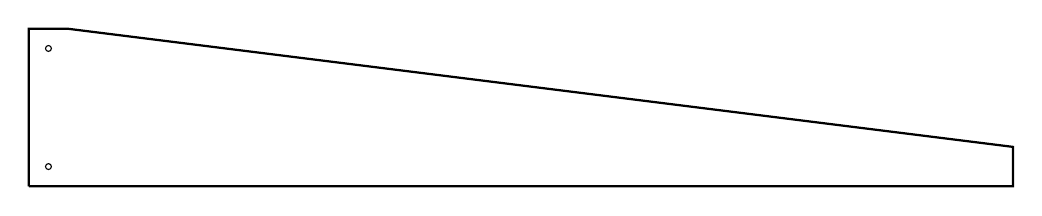
\begin{tikzpicture}
% draw top
\draw[thick] (0,0) -- (12.5,0) -- (12.5,0.5) -- (0.5,2) -- (0.0,2) -- (0,0);
\draw (0.25,0.25) circle (0.375mm);
\draw (0.25,1.75) circle (0.375mm);
\end{tikzpicture}
\caption{Wings front, rear, bottom and side view.}
\label{fig:wings}
\end{figure}
\begin{figure}[h]
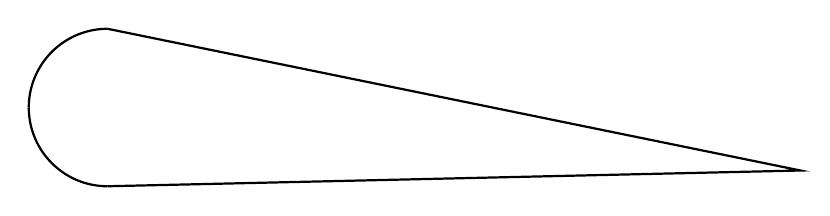
\begin{tikzpicture}
% draw airfoil
\draw[thick] (0.2,3) arc (180:90:10mm);
\draw[thick] (1.2,2) arc (270:180:10mm);
\draw[thick] (1.2,2) -- (10,2.2) -- (1.2,4);
\end{tikzpicture}
\caption{Airfoil of the wing.}
\label{fig:airfoil}
\end{figure}
\newpage
\subsubsection{Stabilizer}
The wing schematics for the vertical and horizontal stabilizer are depicted in figure \ref{fig:wings_stab}.
\begin{figure}[h]
\begin{tikzpicture}
% draw horizontal
\draw[thick] (0,0) -- (12,0) -- (12,2) -- (1,5) -- (0,5) -- (0,0);
\hole{0.5}{0.5}{1.5};
\hole{0.5}{4.5}{1.5};
\draw[densely dotted] (-0.2,0.5) -- (0.3,0.5);
\draw[densely dotted] (-0.2,4.5) -- (0.3,4.5);
\draw[densely dotted] (0.5,-0.3) -- (0.5,0.3);
\draw[densely dotted] (0.5,0.7) -- (0.5,4.3);
\draw[densely dotted] (1.0,-0.3) -- (1.0,5);

\dimsv{0.0}{0.5}{-0.4};
\dimsv{0.5}{4.5}{-0.4};
\dimsv{4.5}{5}{-0.4};

\dimsv{0.0}{2.0}{12.4};

\dimsh{0.0}{0.5}{-0.4};
\dimsh{0.5}{1.0}{-0.4};
\dimsh{1.0}{12}{-0.4};

% draw vertical
\draw[thick] (0,8) -- (15,8) -- (15,10) -- (1,13) -- (0,13) -- (0,8);
\hole{0.5}{8.5}{1.5};
\hole{0.5}{12.5}{1.5};
\draw[densely dotted] (-0.2,8.5) -- (0.3,8.5);
\draw[densely dotted] (-0.2,12.5) -- (0.3,12.5);
\draw[densely dotted] (0.5,7.7) -- (0.5,8.3);
\draw[densely dotted] (0.5,8.7) -- (0.5,12.3);
\draw[densely dotted] (1.0,7.7) -- (1.0,13);

\dimsv{8.0}{8.5}{-0.4};
\dimsv{8.5}{12.5}{-0.4};
\dimsv{12.5}{13}{-0.4};

\dimsv{8.0}{10.0}{15.4};

\dimsh{0.0}{0.5}{7.6};
\dimsh{0.5}{1.0}{7.6};
\dimsh{1.0}{15}{7.6};

\end{tikzpicture}
\caption{Vertical (top) and horizontal (bottom) stabilizer wings.}
\label{fig:wings_stab}
\end{figure}
\end{document}